\documentclass[11pt,onside]{report}
\usepackage{a4}
\usepackage[a4paper,inner=1.5cm,outer=1.5cm,tmargin=3cm, bmargin=3cm,headsep=1.0cm,bindingoffset=0cm,headheight=14pt]{geometry}
\usepackage[onehalfspacing]{setspace}
\usepackage[utf8]{inputenc}
\usepackage[american]{babel}
\usepackage{fancyhdr}
\pagestyle{fancy}
\fancyfoot[C]{\vspace{3pt} \thepage}
\usepackage[titletoc]{appendix}



\usepackage{multirow}
\usepackage[bf,format=plain]{caption}
\usepackage{xcolor}
\usepackage{graphicx}
\usepackage{wallpaper}
\usepackage{wrapfig}
\usepackage{subfig}
\captionsetup[subfloat]{labelfont={footnotesize,rm,md,up}}
\usepackage{float}
\usepackage{longtable}
\usepackage{booktabs}
% \usepackage{icomma}
\usepackage{tablefootnote}
\usepackage{enumitem}

\usepackage{latexsym,exscale,amssymb,amsmath,amsfonts,amstext,amsbsy,esint}
\usepackage[thinspace,thickqspace,squaren]{SIunits}

% \usepackage[crop=pdfcrop]{pstool}

% \usepackage{lscape}

% \usepackage[square,numbers,sort&compress]{natbib}
\usepackage[babel]{csquotes}
% \usepackage[
  % backend=biber,
  % bibstyle=numeric,
  % citestyle=numeric-comp,
  % firstinits=true,
  % maxcitenames=1,
  % maxbibnames=99,
  % date=short,
  % isbn=false,
  % url=false,
  % eprint=true,
  % sorting=none,
  % sortcites=true]{biblatex}
% \addbibresource{literatur.bib}

% \renewbibmacro*{volume+number+eid}{%
  % \textbf{%
  % \printfield{volume}}%
  % \setunit*{\addnbthinspace}%
  % \printfield{number}%
  % \setunit{\addcoma\space}%
  % \printfield{eid}}%
% \DeclareFieldFormat[article]{number}{\mkbibparens{#1}}
% \renewbibmacro{in:}{}

% \renewbibmacro*{issue+date}{%
% %   \setunit{\addcomma\space}% NEW
% %  \printtext[parens]{% DELETED
    % \iffieldundef{issue}
      % {\printfield{year}}
      % {\printfield{issue}%
       % \setunit*{\addspace}%
% %       \usebibmacro{date}}}% DELETED
       % \printfield{year}}% NEW
  % \newunit}


\usepackage[
bookmarks=true,
allcolors=black,
allbordercolors=black,
colorlinks=true,
linkcolor=black,
pdfauthor={Jan Thiart, Simon Christoph Stein},
pdftitle={TrackNTrace - Manual},
pdfsubject={Manual},
pdfcreator={Jan Thiart},
pdfkeywords={}]
{hyperref}

%%%%%%%%%%%%%%%%%%%%%%%%%% Definitionen %%%%%%%%%%%%%%%%%%%%%%%%%%


\newcommand{\D}[0]{\text{d}}
\newcommand{\N}{\ensuremath{{\vec{\nabla}}}}
\newcommand{\laplace}{\ensuremath{{\underline{\Delta}}}}
\newcommand{\ssection}[1]{\vspace{5mm} \section{#1}}
\newcommand{\ssubsection}[1]{\vspace{5mm} \subsection{#1}}
\newcommand{\scite}[1]{\citep{#1}}
\renewcommand*{\vec}[1]{\ensuremath{\mathrm{\mathbf{{#1}}}}}
\newcommand*{\svec}[1]{\ensuremath{\boldsymbol{{#1}}}}



\numberwithin{equation}{chapter}
% \numberwithin{figure}{chapter}
\renewcommand{\thesection}{\arabic{section}}


% \renewcommand*\thefigure{\thesection.\arabic{figure}}
\renewcommand*\thesubfigure{\alph{subfigure}}
\makeatletter
\renewcommand\p@subfigure{\thefigure}
\makeatother
\setcounter{lofdepth}{2}

\makeatletter
\renewcommand{\paragraph}{\@startsection{paragraph}{4}{\z@}%
  {-3.25ex\@plus -1ex \@minus -.2ex}%
  {1.5ex \@plus .2ex}%
  {\normalfont\normalsize\bfseries}}
\makeatother

\setcounter{secnumdepth}{5}
\setcounter{tocdepth}{5}





% \parindent0mm

\hyphenation{TrackNTrace}

\newcommand{\executeiffilenewer}[3]{%
\ifnum\pdfstrcmp{\pdffilemoddate{#1}}%
{\pdffilemoddate{#2}}>0%
{\immediate\write18{#3}}\fi%
}
\newcommand{\includesvg}[1]{%
\executeiffilenewer{#1.svg}{#1.pdf}%
{inkscape -z -D --file=#1.svg %
--export-pdf=#1.pdf --export-latex}%
\input{#1.pdf_tex}%
}




\makeatletter
\gdef\tshortstack{\@ifnextchar[\@tshortstack{\@tshortstack[c]}}
\gdef\@tshortstack[#1]{%
  \leavevmode
  \vtop\bgroup
    \baselineskip-\p@\lineskip 3\p@
    \let\mb@l\hss\let\mb@r\hss
    \expandafter\let\csname mb@#1\endcsname\relax
    \let\\\@stackcr
    \@ishortstack}
\makeatother


\def\CC{{C\nolinebreak[4]\hspace{-.05em}\raisebox{.4ex}{\tiny\bf ++}}}



%%%%%%%%%%%%%%%%%%%%%%%%%%%%% Inhalt %%%%%%%%%%%%%%%%%%%%%%%%%%%%%

\begin{document}
\chapter*{TrackNTrace}
\vspace*{-30pt}\textbf{written for Matlab by Simon Christoph Stein and Jan Thiart}\\ [20pt]
TrackNTrace is a fast, easy-to-use Matlab program created for locating bright, Gaussian-shaped spots in a 2D fluorescence microscopy image or movie and track such emitters over time. It can be used in localization microscopy (PALM, STORM, ...), Single-molecule Particle Tracking (SPT), for drift correction and similar applications and comes with a convenient interface for configuration. Locating and tracking fluorescent emitters is done in two separate steps and it is comparatively easy to everyone with basic Matlab knowledge to alter the respective scripts, e.g. to include additional tracking algorithms. TrackNTrace should be useful to anyone who seeks to combine the speed of established software packages such as RapidSTORM or quickPALM with the simplicity and direct modifiablity of Matlab, especially when further post-processing is also done in Matlab.\\
In general, TrackNTrace reads a movie file, corrects for camera artifacts if applicable and obtains a rough guess of all possible positions of bright spots in every image. These position candidates then serve as the basis for a fitting routine which fits a 2D Gaussian bell curve to the pixel intensity values around each candidate as an approximation of the microscope Point Spread Function (PSF), obtaining position, amplitude and local background. Finally, these fit results are then returned to a particle tracking algorithm which tries to link particles close in time and space to form trajectories.\\[10pt]
This manual will first provide all necessary steps for installation (section~\ref{sec:install}) and explain the configuration utility (section~\ref{sec:config}). Some in-depth information about the operation of TrackNTrace is provided in section~\ref{sec:in-depth}.
\begin{table}[!h]
\centering
\caption*{\textbf{Requirements}}
\label{tab:requirements}
\begin{tabular}{p{.2\textwidth} p{.45\textwidth}}
\toprule
OS & Windows 7 64-bit or higher\tablefootnote{Necessary libraries can also be compiled for Linux and Mac.} \\[5pt]
Matlab version & 2009a or higher\\[5pt]
Toolboxes & Image Processing, Statistics \\[0pt]
\bottomrule
\end{tabular}
\end{table}

Please also note: TrackNTrace currently can only handle single-channel, $\mathrm{2D}+\mathrm{t}$ Tif image stacks. Convert your experimental data accordingly. \clearpage%

\section{Installation}\label{sec:install}
Installation procedure for Windows 7:
\begin{enumerate}
\item Extract \texttt{TrackNTrace.zip} to your Matlab root path directory (e.g. \url{C:\\Users\\\%USERNAME\%\\Documents\\MATLAB}).
\item Open the TrackNTrace folder and run \texttt{vcredist\_x64.exe}.
\item Open Matlab and go to the TrackNTrace folder.
\item Run \texttt{RunTrackNTrace.m}.
\end{enumerate}

\section{Configuration}\label{sec:config}
When you first run \texttt{RunTrackNTrace.m}, the GUI as seen in figure~\ref{subfig:settings-gui} pops up. Here, you can select the relevant movie files to process, set options to find spots and fit a PSF model to them, and handle the particle tracking algorithms. All relevant file names, options, particle locations, and trajectories are stored in a time-stamped \texttt{mat}-file whenever they become available which makes it very easy to repeat and compare different experiments and very hard to lose any progress. Before processing begins, users can enable a preview mode to try and optimize different settings, either individually for all selected movies or globally. Finally, finished movies can be inspected in Matlab with trajectories overlaid.\\
You can always save the current settings in a different \texttt{mat}-file and load them at the start by clicking on \textsf{Save Settings} and \textsf{Load settings}, respectively. In such a case, one only needs to select the movies to process and can skip anything else. Clicking on \textsf{Continue \& use for all} will use the same settings for all selected movies while clicking \textsf{Continue} will invoke the GUI again for each individual movie.

\subsection*{General options}
\begin{itemize}[leftmargin=2cm]
\item[Movie list] Click on \textsf{Select} to open a file dialogue where you can select one or multiple movies to analyze.
\item[Dark movie] Select a movie taken with the exact same camera settings used in your experiment but with the shutter closed. This movie is used to correct for non-isotropic camera sensitivity, dead pixels and other artifacts according to [1].
\item[Frame interval] Select the first and the last movie frame for processing. Anything not in this interval will be discarded. If \textsf{Last frame} is higher than the movie size or set to \textsf{Inf}, the whole movie is processed, starting at \textsf{First frame}.
\item[Preview mode] Enable previw mode and select its frame interval. If you click \textsf{Continue} and preview mode is enabled, all current settings will be applied to analyze a portion of the movie (keep the frame interval between 50 and 100 frames to avoid performance drops). A movie player (see fig.~\ref{subfig:preview},\ref{subfig:preview2}) will pop up where you can see all positions, and trajectories if tracking was enabled, which are the result of the settings you choose. This is very useful for fine-tuning all relevant options before starting analysis on the whole movie.\\
Please note: Additional preview options are available when leaving \textsf{Tracking} disabled. In this case. fig.~\ref{subfig:preview2} shows up and you have additional filtering options for amplitude and SNR. On top of that, you can also plot histograms of the fitted amplitudes, background counts, and PSF standard deviations which, for example, enables you to first fit the PSF, choose an appropriate value, and fit (and track) the rest of the movie with a fixed PSF standard deviation.\\
Once you close the preview window, you will get asked to continue testing or abort the preview. Clicking \textsf{Yes} takes you back to the settings GUI, \textsf{No} acknowledges your satisfaction with the current settings and continues with the next film.
\end{itemize}

\begin{figure}[!h]
\centering
\subfloat[][GUI for TrackNTrace settings.]{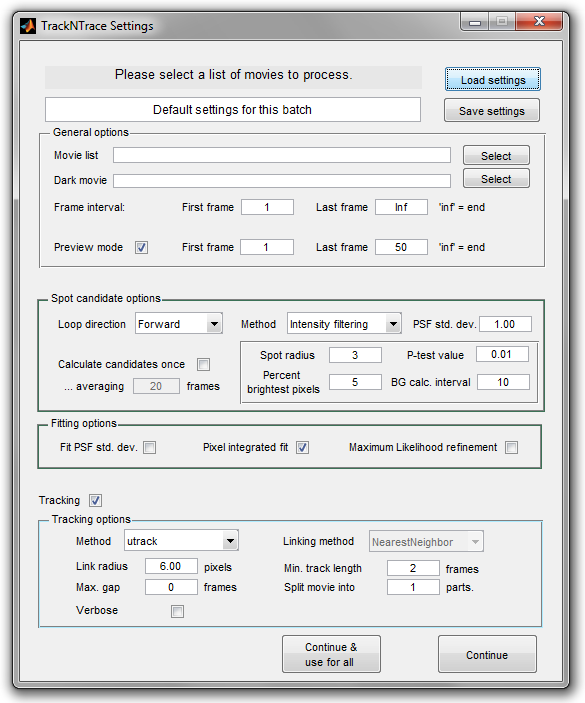
\includegraphics[width=5.95cm]{./settings_gui_first.png} \label{subfig:settings-gui}} \qquad
\subfloat[][GUI for trajectory preview.]{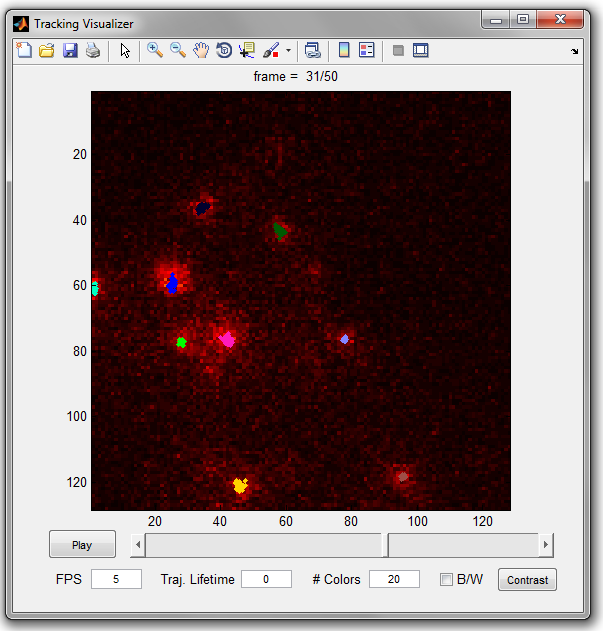
\includegraphics[width=6.88cm]{./preview_gui.png} \label{subfig:preview}}\\
\subfloat[][GUI for positions preview with a histogram of fitted PSF standard deviations.]{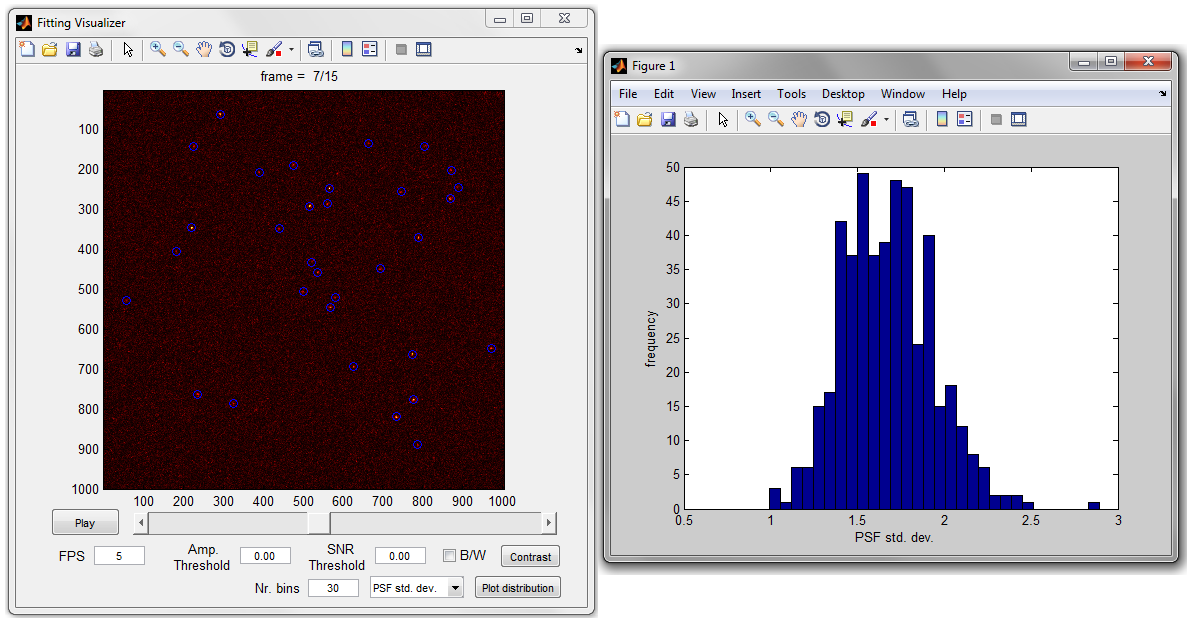
\includegraphics[width=12.88cm]{./fitdata_visual.png} \label{subfig:preview2}}\\
\caption{TrackNTrace GUIs.}
\end{figure}

\subsection*{Spot candidate/Fitting options}
Here, you can control how to roughly identify bright spots in your movies. These spot candidates are later fit and accurate positions and amplitudes get extracted. 
\begin{itemize}[leftmargin=2cm]
\item[Loop direction] Movies can be processed in a forward direction, from beginning to end, or backwards. Normally, there is no difference between the two. However, this setting can be used in combination with \textsf{Calculate candidates once} (see below).
\item[\smash{\tshortstack[1]{Calculate candi-\\dates once}}] If enabled, spots are only detected once from an average over the first (or last, with \textsf{Loop direction = Backward}) $N$ frames of the movie. The number of frames $N$ can be adjusted below the checkbox. Instead of independent spot detection \& fitting for every frame, the fit results of the last frame are carried over as an initial guess for the next frame. Useful for drift correction or blinking/bleaching analysis of non-moving particles at low signal to noise.
\item[Method] Choose the method used to find spot candidates, which can be intensity filtering or cross-correlation. The former works well in any case while the latter is very useful if looking at non-moving diffraction limited emitters.
\item[PSF std. dev.] TrackNTrace assumes an isotropic Gaussian PSF model for fluorescent emitters [2], where the provided value is the Gaussian standard deviation $\sigma$ in pixels. A lower bound can be calculated as $\sigma = \frac{\lambda_\mathrm{em}}{4\sqrt{2\ln 2}\: \mathrm{NA}}$, where $\lambda_\mathrm{em}$ is the fluorescence emission wavelength in pixels and NA is the numerical aperture of the microscope. This number is especially important when using cross-correlation. Use the positions preview (\textsf{Tracking} disabled) to check the distribution of fitted $\sigma$ to set an appropriate value.
\item[Spot radius] Average radius of a spot in pixels, must be an integer.
\item[\smash{\tshortstack[1]{Percent brightest\\ pixels}}] Only the brightest $q\%$ of all pixels can be considerred as candidates. Lower means less candidates but higher candidate amplitude.
\item[P-test value] Every emitter's brightness is compared to its background via a hypothesis test, with the background assumed to be Gaussian. Lower means less candidates but higher candidate amplitude. Must be between 1 and 0.
\item[BG calc. interval] This setting forces a new local background image to be calculated every $n$ frames. Setting a low number results in higher quality localizations at the cost of a severely reduced performance.
\item[Threshold] This number $t$ is only used in the cross-correlation step and must be between 1 and 0. Choosing a large value for $t$ will make sure only spots which strongly match the Gaussian PSF model are chosen as spot candidates.\\[0pt]%
%
\item[Fit PSF std. dev.] This enables fitting the PSF standard deviation on top of position, amplitude and background. Useful for wide particle size distributions or diffusing molecules.
\item[Pixel integrated fit] Enables or disables fitting a Gaussian model integrated over one pixel. It more accurately resembles the process of photons hitting the discrete pixel grid of a camera chip surface and is recommended to be enabled [2].
\item[\smash{\tshortstack[1]{Maximum Likeli- \\hood refinement}}] If enabled, the fitting algorithm uses a combination of Least-squares Minimization and Maximum Likelihood Estimation [2] for parameter optimization.
\end{itemize}

\subsection*{Tracking options}
This section contains all settings relevant to particle tracking. Tracking can also be disabled altogether by unticking \textsf{Tracking}.

\begin{itemize}[leftmargin=2cm]
\item[Method] Choose the tracking algorithm you would like to use. Possible methods at this point are \textsf{u-track} [3], and a custom nearest-neighbor tracker written in \CC.
\item [Link radius] Maximum allowed distance a particle can travel between two frames. A good setting for diffusing particles is $3\sqrt{2 D t_a}$, where $D$ is the diffusion coefficient and $t_a$ is the frame aquisition time.
\item [Max. gap] Maximum amount of frames a particle can be invisible (e.g. by entering a non-radiative triplet state) between two observations without ending the trajectory prematurely. While useful for stationary, blinking fluorophores, allowing gaps for diffusing particles can severely distort the result. Set to 0 to disable.
\item [Min. track length] All trajectories shorter than the minimum allowed track length will be discarded automatically. 
\item [\smash{\tshortstack[1]{Split movie\\into parts}}] Particle tracking can be very memory-intensive and taxing on the CPU when dealing with a large amount of frames and particles, especially when gap closing is enabled. As performance does not scale linearly, splitting the movie into 2 or more parts can boost performance considerably. Choose with care if you do not want to allow tracks being split into smaller segments, e.g. when large gap closing values were chosen.
\item [Verbose] If enabled, progress updates will be displayed if the tracking algorithm supports it.
\end{itemize}
\clearpage
\section{TrackNTrace data structures}
All results obtained by TrackNTrace are saved in a \texttt{mat}-file in the format \texttt{'moviename\_timestamp\_TNT.mat'}. Here is a list of all variables it contains:
\begin{table}[!h]
\centering
\caption*{\textbf{TrackNTrace data structures}}
\label{tab:datastruct}
\begin{tabular}{p{.25\textwidth} p{.7\textwidth}}
\toprule
\multicolumn{1}{c}{Variable name} & \multicolumn{1}{c}{Description}\\ \midrule
\texttt{filename\_movie} & String containing full path of movie file. \\[5pt]
\texttt{dark\_img} & 2D double array containing correction image to be added to each movie frame. \\[5pt]
\texttt{generalOptions} & $1\times1$ struct of general options variables set by the GUI. \\[5pt]
\texttt{candidateOptions} & $1\times1$ struct of candidate options variables set by the GUI. \\[5pt]
\texttt{fittingOptions} & $1\times1$ struct of fitting options variables set by the GUI. \\[5pt]
\texttt{trackingOptions} & $1\times1$ struct of general options variables set by the GUI. \\[5pt]
\texttt{fitData} & $n\times 1$ cell array of fitted positions where $n$ is the number of analyzed frames. Each cell contains a $k\times p$ double array, where $p$ is the number of model parameters and $k$ is the maximum amount of particles in the respective frame. Each row represents a unique fit and the column order according to the model PSF is $\mu_x$, $\mu_y$, $A$, $B$, $\sigma$ and $\varepsilon$ (see sec~\ref{sec:in-depth} for details). $\varepsilon$ is a flag set by the fitting routine indicating if a fit converged ($\varepsilon = 1$) or not ($\varepsilon = -1$), or if the fit failed altogether ($\varepsilon = -2$) Currently, failed fits are not saved at all. \\
 & For example, \texttt{fitData\{f\}(:,1:3)} shows a list of all valid particles in frame $f$ in row order with $xy$ position and amplitude as columns.\\[5pt]
\texttt{trajectoryData} & 2D double array of all trajectories. Each trajectory is assigned a unique id after which the array is sorted. The column order is id, frame, $\mu_x$, $\mu_y$, $A$. Both id and frame begin at 1. \\
\bottomrule
\end{tabular}
\end{table}

\section{How TrackNTrace works}\label{sec:in-depth}
After storing all options, reading in the movie and, if applicable, a closed shutter movie for correction, the fitting routine starts. First, the movie frame is cleaned up by adding a correction image obtained from the closed shutter movie as described in [1]. Then, the respective candidate search function is called for the respective frame and the result is passed to the fit function. Depending on the settings, candidate search is carried out in each frame or only once for the first (or last) frame or an average image of the first few (or last few) frames. In the latter case, fit results from the frame before are passed to the fit function in the next iteration. \\
Two candidate search mechanism are possible: Normalized cross-correlation and intensity filtering. For cross-correlation, a Gaussian PSF mask is created and the \texttt{normxcorr2} function is called to calculate a correlation image of the original movie frame. This image is then processed with a local maximum filter using \texttt{imdilate}. Pixels with a correlation value higher than the user-provided threshold are accepted as spot candidates. In the intensity filtering step, the image is convolved with a normalized filter kernel  consisting of a moving average window and a Gaussian bell curve of $\sigma = \unit{1}{\mathrm{px}}$ against discretization noise before being processed with a local maximum filter. The kernel has a window size of $w = 2r+1$ where $r$ is the spot radius given by the user. Next, a local background image [4] is calculated and all pixels have to pass two tests: The intensity must be among the top $q\%$ in the image and $1-\mathrm{CDF}(\mu_b,\sigma_b) \leq p$ must hold, where CDF ist the normal distribution cumulative density function, and $\mu_b$ and $\sigma_b$ are mean and standard deviation of the local background. $p$ and $q$ are user-provided thresholds.\\[10pt]
A list of spot candidate positions is passed to a \texttt{Mex} file which handles all fitting procedures. First, a square quadrant $I_\mathrm{exp}$ around a candidate pixel is fit to a 2D Gaussian,
\begin{align*}
I_\mathrm{theo}(x,y) = A\exp\left(-\frac{(x-\mu_x)^2}{2\sigma^2} - \frac{(y-\mu_y)^2}{2\sigma^2}\right) + B \quad\mathrm{with}\quad \min_\theta \sum_x\sum_y \left(I_\mathrm{theo}-I_\mathrm{exp}\right)^2
\end{align*}
where $\theta = (A,\mu_x,\mu_y,B,\sigma)$. Fitting $\sigma$ can be disabled by the user. A more accurate model can be obtained by taking into account the finite size of the camera chip pixel grid, where all signal photons hitting any point within a square pixel are accumulated:
\begin{align*}
I_\mathrm{theo, px} &= \int\limits^{+1\slash 2}_{-1\slash 2} \D x \int\limits^{+1\slash 2}_{-1\slash 2} \D y\: I_\mathrm{theo} \\
&= \frac{A \pi \sigma^2}{2}\cdot \left[\mathrm{erfc}\,\left(-\frac{x-\mu_x+1\slash 2}{\sqrt{2} \sigma}\right) - \mathrm{erfc}\,\left(-\frac{x-\mu_x-1\slash 2}{\sqrt{2} \sigma}\right)\right] \times \\
&\quad \left[\mathrm{erfc}\,\left(-\frac{y-\mu_y+1\slash 2}{\sqrt{2} \sigma}\right) - \mathrm{erfc}\,\left(-\frac{y-\mu_x-1\slash 2}{\sqrt{2} \sigma}\right)\right] +B
\end{align*}
Here, $\mathrm{erfc}$ is the complementary error function. Note that $x$- and $y$- dimension are decoupled, meaning that the two terms only have to be calculated once for one column and one line. Residual minimization is done by a Least-squares Levenberg-Marquardt algorithm. The result can be fitted again using Maximum Likelihood Estimation which is proven to yield the best possible result [2]:
\begin{align*}
\min_\theta (-\log\mathcal{L}) = \min_\theta (I_\mathrm{theo}(\theta) - I_\mathrm{exp} \ln I_\mathrm{theo}(\theta))
\end{align*}
All optimization steps rely on the \texttt{ceres-solve}r library, an open-source optimization library written in \CC by Google Inc. We chose ceres for its very high performance, great customizability and the possibility of calculating all necessary first-order derivatives by using automatic differentiation which does not require user input and is therefore more robust. The matlab implementation by Simon Christoph Stein is available on the Matlab file exchange where you can also find all necessary files and instructions for building {TrackNTrace}:  \texttt{http://www.mathworks.com/matlabcentral/fileexchange/52417-fast-gaussian-point-spread-\\function-fitting--mex-}\\[10pt]
% FIXME \url did not break the url properly, even after trying different options/packages for 20 minutes.. (latex, *rolleyes*)
 After fitting is finished and if tracking is enabled, the result array is converted to a format suitable for the chosen tracker and passed to the tracking routine. Currently there are two options available: u-Track [3], and a custom, highly efficient nearest-neighbor tracker written in \CC. Depending on the tracker, the time complexity of particle linking is at least quadratic in the number of particles, linear in the number of frames and quadratic or even exponential in the number of gap frames. In u-Track's case, splitting the movie into several parts can be much faster than processing all positions in a single batch. In such situations, particles within and directly after such a border or split frame are tracked again to try to re-link trajectory segments artificially cut in half by splitting the movie. Gap frames cannot be accounted for in this case, therefore, caution is advised when using larger gap values and splitting numbers together.\\
For every tracker, the end result is an array containing all trajectories with recorded frame number, and respective $xy$- position and amplitude. Every trajectory has a unique id to facilitate post-processing. \\
While all tracking algorithms are handled more or less the same, u-Track is an exception. u-Track can handle very difficult scenarios such as Brownian-directional motion-switching, particle merging and splitting and provides a large number of user-input variables for this. These options are all hidden in the \texttt{parseUtrackOptions.m} file and are only meant to be changed by an experienced user. Caution is advised.




\section{References}
\begin{itemize}
\item [{[1]}]  Hirsch M, Wareham RJ, Martin-Fernandez ML, Hobson MP, Rolfe DJ: A Stochastic Model for Electron Multiplication Charge-Coupled Devices – From Theory to Practice. PLoS ONE 8(1), 2012.
\item [{[2]}] Mortensen, KI, Churchman SL, Spudich, JA, Flyvbjerg H: Optimized localization analysis for single-molecule tracking and super-resolution microscopy. Nature Methods 7, 377 - 381, 2010.
\item [{[3]}] Jaqaman K et al: Robust single-particle tracking in live-cell time-lapse sequences. Nature Methods 5, 695 - 702, 2008.

\end{itemize}



\end{document}

















































